\documentclass[aspectratio=169,10pt]{beamer}
\usetheme{Madrid}
\usecolortheme{default}
\usepackage{amsmath,amssymb}
\usepackage{tikz}
\usetikzlibrary{positioning,arrows.meta,shapes.geometric}
\usepackage{booktabs}
\usepackage{xcolor}
\usepackage{tabularx}

\definecolor{uavblue}{RGB}{37,99,235}
\definecolor{uavgreen}{RGB}{22,163,74}
\definecolor{uavred}{RGB}{220,38,38}
\definecolor{uavorange}{RGB}{234,88,12}
\definecolor{uavgray}{RGB}{71,85,105}
\definecolor{uavlight}{RGB}{241,245,249}

\title{Persistent K-Coverage: Where the Progress Really Stands}
\subtitle{Professor progress meeting --- 4 November 2026}
\author{Himanshu Nagwanshi, Surya Prakash S, Harsh Varshney, Gaddam Viswavijith}
\date{}

\begin{document}

\begin{frame}
  \titlepage
\end{frame}

\begin{frame}{Agenda (15 minutes)}
  \begin{enumerate}
    \item What the report is now
    \item What we fixed, and what we hid nowhere
    \item The measured headline: where learning wins and loses
    \item The energy-flow certificate
    \item Planning oracle and the deployable distilled policy
    \item Honest verdict, risks, and what we need from you
  \end{enumerate}
\end{frame}

\begin{frame}{What the report is now}
  \begin{itemize}
    \item 27 pages; title changed to \emph{``Energy-Flow Feasibility and Learned Redundancy Management for Persistent K-Coverage UAV Networks''}.
    \item Story order: certificate $\rightarrow$ controller $\rightarrow$ honest negatives.
    \item Frozen policy; held-out scenes (seeds $\ge 1000$); paired 95\% intervals.
    \item Bug story moved to the appendix; the headline number is the corrected one.
  \end{itemize}
  \vspace{0.2cm}
  {\scriptsize
  \textbf{The evaluated observation is 68-dimensional}

  \texttt{30 base} + \texttt{16 map grid} + \texttt{8 agent ID}
  + \texttt{3 pad bearing} + \texttt{11 ego-centric deficit bearings}

}
\end{frame}

\begin{frame}{What broke, and what fixed it}
  \begin{center}
  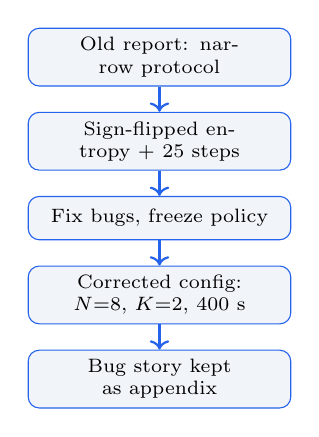
\begin{tikzpicture}[node distance=0.32cm, every node/.style={rounded corners, fill=uavlight, draw=uavblue, minimum height=0.55cm, text width=3.1cm, align=center, font=\scriptsize}]
    \node (old) {Old report: narrow protocol};
    \node[below=of old] (bug) {Sign-flipped entropy + 25 steps};
    \node[below=of bug] (fix) {Fix bugs, freeze policy};
    \node[below=of fix] (cfg) {Corrected config: $N{=}8$, $K{=}2$, $400$~s};
    \node[below=of cfg] (app) {Bug story kept as appendix};
    \draw[->, thick, uavblue] (old) -- (bug);
    \draw[->, thick, uavblue] (bug) -- (fix);
    \draw[->, thick, uavblue] (fix) -- (cfg);
    \draw[->, thick, uavblue] (cfg) -- (app);
  \end{tikzpicture}
  \end{center}
\end{frame}

\begin{frame}{Measured headline (report)}
  \begin{center}
  \scriptsize
  \begin{tabular}{lcc}
    \toprule
    Comparison & CK & Notes \\
    \midrule
    MAPPO (ego + shaping) & 0.9512 & held-out, 20 scenes \\
    Strongest rule (Reactive-local) & 0.923 & +0.028, CI excludes zero \\
    Oracle ceiling & 1.000 & oracle placement, identical for all \\
    Classical OR scheduler & 0.929 & oracle + Hungarian + rotation \\
    \bottomrule
  \end{tabular}
  \end{center}
  \vspace{0.18cm}
  \begin{itemize}
    \item Learning is ahead on nominal and low connectivity; behind on small battery and spread start.
    \item Bug-fixes-only: 0.859; anchor ego+shaping: 0.9512.
  \end{itemize}
\end{frame}

\begin{frame}{Stress regimes (5 held-out scenes)}
  \begin{center}
  \small
  \begin{tabular}{lcccc}
    \toprule
    Regime & Best rule & MAPPO & Classical OR & MAPPO $-$ rule \\
    \midrule
    nominal & 0.921 & 0.947 & 0.929 & +0.026 \\
    small battery & 0.829 & 0.765 & 0.791 & $-0.064$ \\
    low comm & 0.804 & 0.928 & 0.808 & +0.125 \\
    spread start & 0.997 & 0.959 & 0.980 & $-0.038$ \\
    failure & 0.912 & 0.946 & 0.919 & +0.034 \\
    multi-failure & 0.910 & 0.945 & 0.919 & +0.035 \\
    \bottomrule
  \end{tabular}
  \end{center}
  \vspace{0.15cm}
  \begin{itemize}
    \item Classical scheduler does not beat the learner in any same-architecture regime.
    \item The strongest win is low connectivity: \,0.928 vs 0.808 (classical) and 0.804 (rule).
  \end{itemize}
\end{frame}

\begin{frame}{Energy-flow certificate (new)}
  \begin{columns}
    \begin{column}{0.48\textwidth}
      \small
      \begin{itemize}
        \item Each of the 2 pads adds 30~W gross, 24.9~W net after avionics.
        \item One airborne UAV draws 55.1~W.
        \item Steady state: only 0.90 UAV can remain airborne.
        \item $K{=}2$ needs 8 UAVs.
      \end{itemize}
    \end{column}
    \begin{column}{0.48\textwidth}
      \small
      \begin{itemize}
        \item Steady-state ceiling = 0.113.
        \item $T{=}400$s: ceiling 1.000 (spends initial packs).
        \item $T{=}2000$s: ceiling 0.367 (full) / 0.326 (mean charge).
        \item Only $N{=}12$, 4 pads, 60~kJ, fast charge achieves 1.000.
      \end{itemize}
    \end{column}
  \end{columns}
  \vspace{0.2cm}
  {\footnotesize \textbf{The reported configuration is not long-horizon persistent.} That is the paper's own, verified finding.}
\end{frame}

\begin{frame}{Planning oracle and the deployable policy}
  \begin{itemize}
    \item Centralised planning oracle: 0.9723 vs base 0.9512.
          Paired +0.0211, CI $[+0.014,+0.028]$, resolved.
    \item It is global, not deployable CTDE.
    \item Distilled 20-epoch actor: 0.9618, paired +0.0106, CI $[-0.002,+0.023]$ (directional).
    \item Planner recoverable as deployable decentralised policy: about half the gain.
    \item Classical OR scheduler: 0.929, still below the learner.
  \end{itemize}
\end{frame}

\begin{frame}{Honest verdict}
  \begin{itemize}
    \item Not a breakthrough; a correct, honest engineering package.
    \item The two ``certificates'' are conservation, not new theory.
    \item The value is the certificate, corrected protocol, and honest negatives.
    \item Realistic venue: NCC / COMSNETS / VTC-ICC workshop / Drones.
    \item Not top-tier (TMC / NeurIPS / ICRA).
  \end{itemize}
  \vspace{0.2cm}
  {\footnotesize The energy certificate makes the paper coherent, not novel in the strongest sense.}
\end{frame}

\begin{frame}{Open issues (we are showing before hiding them)}
  \begin{enumerate}
    \item \textbf{Observation documentation bug:} the report text describes the observation incorrectly; the evaluated 68-dim model includes map grid, agent ID, pad bearing and ego features.
    \item \textbf{Not long-horizon persistent:} the current 400~s scope must stay explicit.
    \item \textbf{Title tension:} energy-first title may invite a rejection before the evidence is read.
    \item \textbf{0.862 ``full coverage'' claim:} provenance and architecture not yet audited.
  \end{enumerate}
\end{frame}

\begin{frame}{What we need from you}
  \begin{enumerate}
    \item Venue scope: regional conference, Drones, or hold until the energy / low-comm story is cleaner.
    \item Title: keep energy-first wording, or move certificate contribution into the abstract and lead with the system.
    \item Scope:\; a) fix documentation and submit as-is;\;\ b) run 2 more experiments (R$_{\mathrm{comm}}$ phase transition; proactive staggered recharging);\;\ c) pivot paper to low$_{\mathrm{comm}}$.
  \end{enumerate}
\end{frame}

\begin{frame}{Next two weeks (proposal)}
  \begin{enumerate}
    \item Fix the observation/config documentation and provenance of 0.862.
    \item $R_{\mathrm{comm}}$ phase-transition sweep with no retraining.
    \item Decide venue and title.
    \item Final submission package: 10 pages + appendix/info-pack.
  \end{enumerate}
\end{frame}

\begin{frame}{Bottom line}
  \textbf{We have a real, corrected, honest contribution, not a breakthrough.}
  \begin{itemize}
    \item Certificate tells us when the task is feasible, including energy.
    \item The learner beats the strongest rule on nominal and low connectivity.
    \item It loses where energy is the constraint; that is the paper's point.
    \item The report is in much better shape, but it still needs one documentation fix before submission.
  \end{itemize}
\end{frame}

\end{document}